%\subsection{Проблемы проектирования}

С помощью построенной расчетной модели, используя существующие расчетные средства (MSC.Nastran), было определено напряженно-деформированное состояние(НДС) БПЛА для минимальных технологических толщин (1мм для алюминиевых панелей). Исходя из полученных данных была проведена оптимизация толщин панелей и стенок отсеков для нахождения минимальной по весу конструкции, удовлетворяющей требованиям прочности.

В полученной модели можно выделить следующие особенности НДС:

\begin{enumerate}
\item Усилия в обшивке фюзеляжа малы за исключением обшивки центроплана. Т.о. большую часть обшивки можно выполнять из более легких, но менее прочных материалов
\item Наибольшие усилия наблюдаются в фюзеляжной части центроплана и в корне крыла. Так, в корне крыла наблюдаются следующие величины усилий: $Q = 13,7~\text{тс}$, $M_\text{изг} = 80~\text{тс}\cdot\text{м}$. Необходимо отдельно рассмотреть влияние искривленной формы центроплана на величину минимально допустимый вес центроплана и возможности уменьшения веса. Такой анализ проведен в Главе \ref{chap:Centroplan}
\item Большие усилия приложены на стенки в местах крепления двигателя (дополнительный анализ этой особенности произведен далее в данном разделе)
\end{enumerate}  


%Обшивка почти не нагружена, можно использовать композиты. Наибольшие напряжения в центроплане - необходим достаточно жесткий короб. Отдельно нужно рассмотреть штаны (на устойчивость рассмотрим сейчас, варианты исполнения в третьей главе) 
%
%В корне крыла Q=13,7тс, Мизг=80 тс*м
%На изломе крыла Q=10,3тс, Мизг=55 тс*м

%В предложенной конструкторами схеме были выявлены некоторые проблемные места, в которых требовался дополнительный анализ. 


\begin{figure}[H]
\centering
\def\svgwidth{0.9\textwidth}
\input{figures/WingDeformation.pdf_tex}
\caption{Эпюра перемещений задней кромки крыла}
\label{fig:WingDeformation}
\end{figure}

 \paragraph{Крепление хвостовой части к кессону центроплана} 
\label{sec:pants}
\begin{figure}[H]
\centering
\def\svgwidth{\textwidth}
\input{figures/IsoviewOfPants.pdf_tex}
%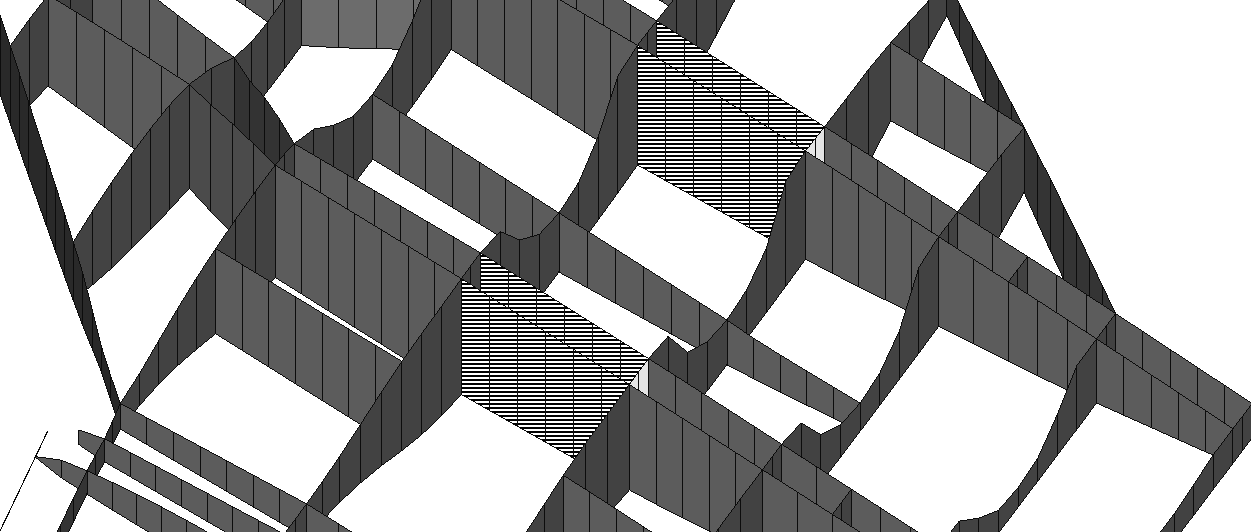
\includegraphics[width=0.6\textwidth]{IsoviewOfPantsBW}
\caption{Вид каркаса фюзеляжа}
\label{fig:IsoviewOfPants}
\end{figure}


Для частичной валидации решения, полученного в результате определния рациональных параметров (см. предыдущий раздел), была решена модельная задача по оценке устойчивости центральных стенок, обеспечивающих крепление хвостовой части гипотетического БПЛА к его центроплану (данные стенки обозначены на Рис.~\ref{fig:IsoviewOfPants} серой заливкой, светло-серой заливкой обозначены зоны основных узлов крепления двигателя). Эти стенки были нагружены перерезывающими усилиями, и необходима была проверка их по условиям устойчивости, которая не проводилась для этих элементов конструкции в процессе определения рациональных параметров. НДС стенок был оценен на основе аналитических формул. Схема нагружения модельных стенок показана на Рис.\ref{fig:IsoviewOfPantsModel}.

\begin{figure}[H]
\centering
%\def\svgwidth{0.9\textwidth}
\input{figures/IsoviewOfPantsModel.pdf_tex}
\caption{Схема нагружения модельных стенок}
\label{fig:IsoviewOfPantsModel}
\end{figure}

%
%\begin{figure}[H]
%\centering
%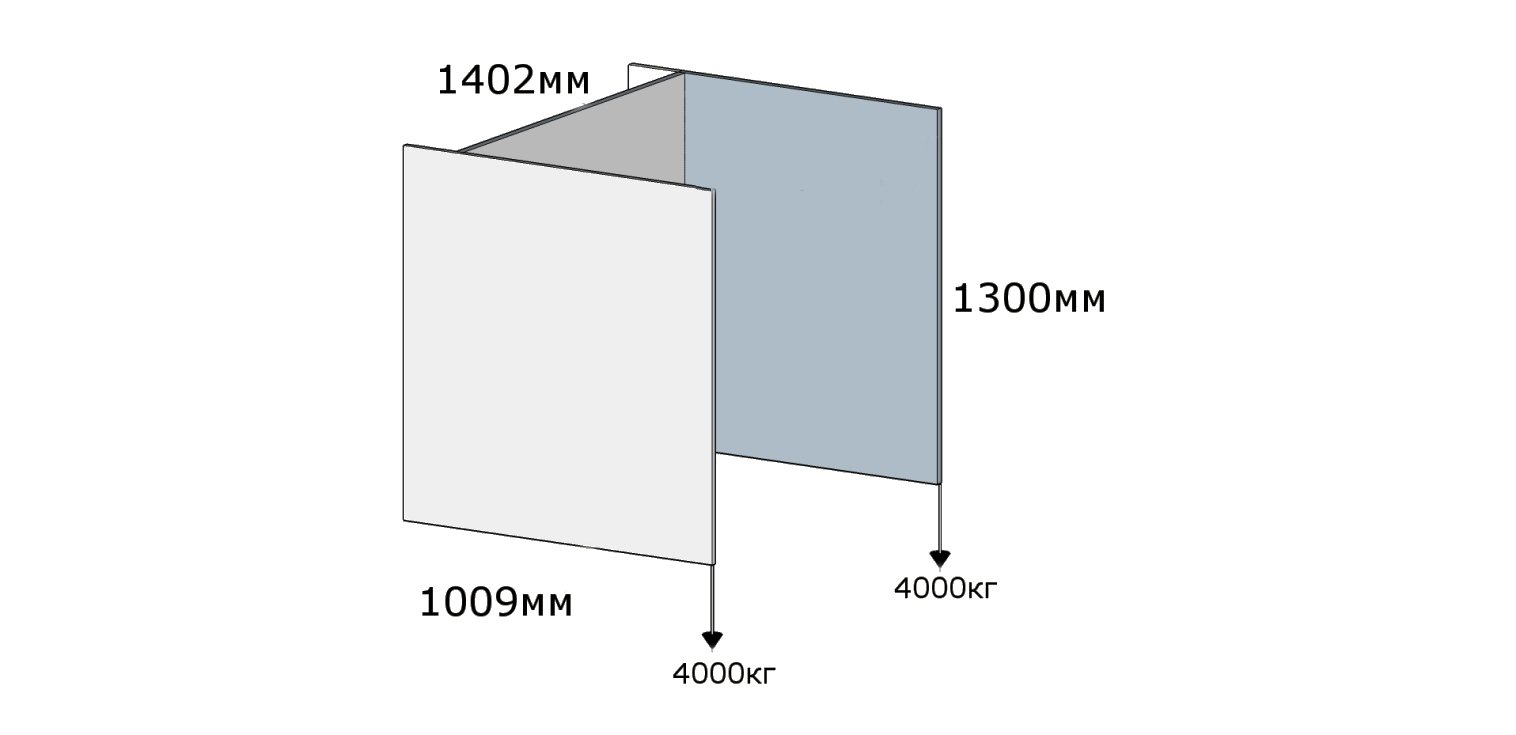
\includegraphics[width=0.8\textwidth]{IsoviewOfPantsModel}
%\caption{Схема нагружения модельных стенок}
%\label{IsoviewOfPantsModel}
%\end{figure}


Уровень нагружения был оценен по величинам касательных напряжений. Касательные напряжения в пластине при чистом сдвиге равны

\begin{equation}
\tau=\frac{3}{2}\cdot\frac{Q}{bh}
\end{equation}
Критические по устойчивости касательные напряжения в пластине при чистом сдвиге равны \cite{Volmir}:

\begin{equation}
\tau_\text{кр}=\frac{K}{12}\frac{\pi^2D}{b^2h} = \frac{K}{12}\frac{\pi^2E}{(1-\mu^2)}\left(\frac{h}{b}\right)^2,\, K=5.34 + 4\frac{a}{b},
\end{equation}
где $a$ - размер пластины вдоль направления действия силы, $b$ - размер пластины поперек направления действия силы, $h$ - толщина пластины, $D$ - изгибная жесткость пластины, $E$ - модуль Юнга, $\mu$ - модуль Пуассона материала пластины, $Q$ - приложенная сила.
Допускаемые толщины найдем из условия:

\begin{equation}
\tau_\text{кр} \geq \tau  
\end{equation}

\begin{equation}
h \geq \sqrt[3]{\frac{3\cdot12}{2}\frac{Qb\cdot(1-\mu^2)}{k\pi^2E}}
\end{equation}

Подставляя значения, получим:

\begin{equation}
Q=\frac{8000}{n}\text{кгс},\,a=1300\text{мм},\,b=1009\text{мм},\,\mu=0.3,\,E=7000\frac{\text{кгс}}{\text{мм}^2}
\end{equation}

\begin{equation}
h \geq \sqrt[3]{\frac{18\cdot8000\cdot1000\cdot(1-\mu^2)}{k\pi^2En}} = \frac{5.67}{\sqrt[3]{n}} 
\end{equation}

Таким образом, для случаев $n = 2$ и $n = 4$  были получены минимальные допустимые толщины, 
равные:

\begin{equation}
h\geq4.50\text{мм},\,n=2
\end{equation}
\begin{equation}
h\geq2.83\text{мм},\,n=4
\label{eq:pants_n4}
\end{equation}

Рациональные значения толщин исследуемых обшивок, полученные в данном проектировочном исследовании, оказались меньше ($h = 1\text{мм}$), чем приведенные в \ref{eq:pants_n4}. Таким образом, выполнение условий по устойчивости этих стенок привело к увеличению их толщин. Более рациональным способом увеличения сдвиговой жесткости этих стенок является использование ферменных подкрепляющих элементов.
%\subsubsection{Фюзеляжная часть центроплана}

Другим проблемным местом была фюзеляжная часть центроплана. Из-за требований компоновки, а именно интеграции двигателя, центроплан необходимо делать изогнутым (Рис.\ref{fig:centroplan}). Это вносит дополнительные трудности в виде увеличения веса по сравнению с прямым центропланом. Исследованию фюзеляжной части центроплана (выделена серым на Рис.\ref{fig:centroplan}) посвящена глава \ref{chap:SolvingModel}.

\begin{figure}[ht]
\centering
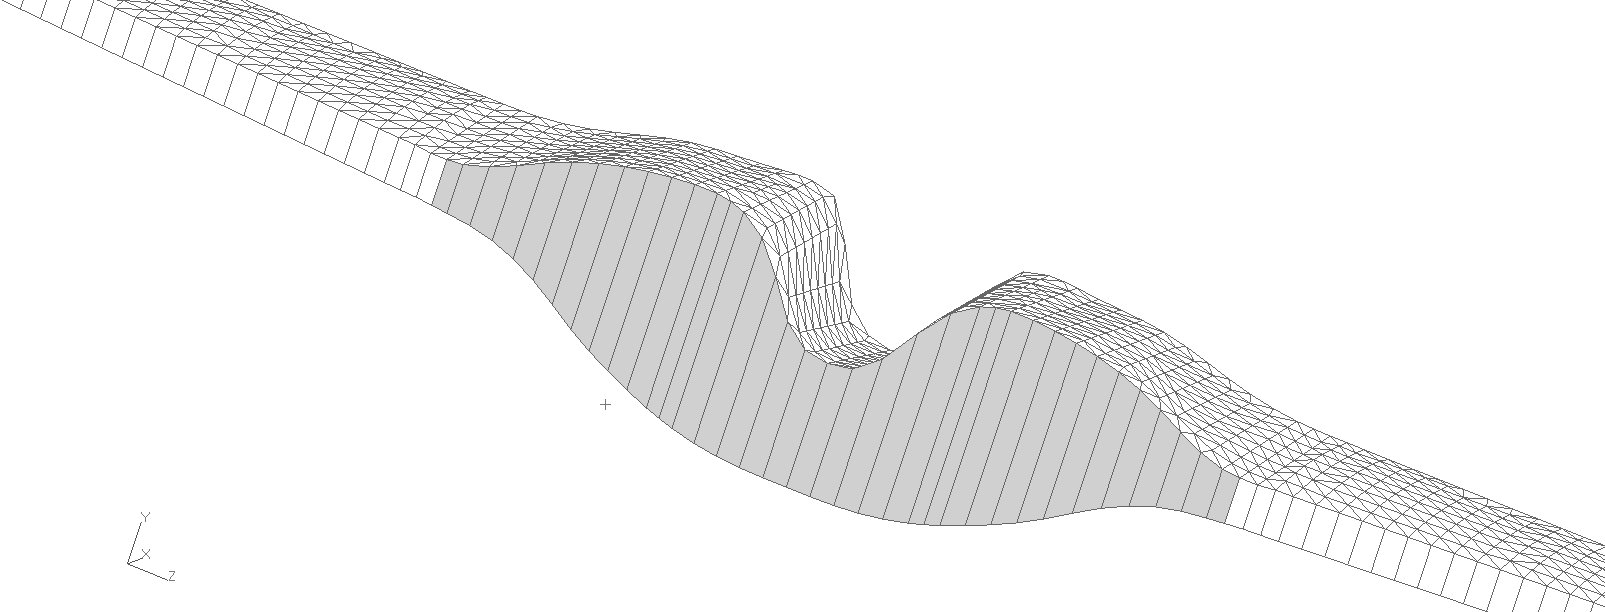
\includegraphics[width=0.6\textwidth]{centroplan}
\caption{Изогнутый центроплан с выделением исследуемой части}
\label{fig:centroplan}
\end{figure}
